\documentclass[a4paper,11pt,final]{article}
        \usepackage{fancyvrb, color, graphicx, hyperref, amsmath, url, textcomp}
        \usepackage{palatino}
        \usepackage[a4paper,text={16.5cm,25.2cm},centering]{geometry}

        %Set different options for xetex and luatex
        \usepackage{iftex}
        \ifxetex\usepackage{fontspec}\fi

        \ifluatex\usepackage{fontspec}\fi

        \usepackage{xcolor}
        % ANSI colors from nbconvert
        \definecolor{ansi-black}{HTML}{3E424D}
        \definecolor{ansi-black-intense}{HTML}{282C36}
        \definecolor{ansi-red}{HTML}{E75C58}
        \definecolor{ansi-red-intense}{HTML}{B22B31}
        \definecolor{ansi-green}{HTML}{00A250}
        \definecolor{ansi-green-intense}{HTML}{007427}
        \definecolor{ansi-yellow}{HTML}{DDB62B}
        \definecolor{ansi-yellow-intense}{HTML}{B27D12}
        \definecolor{ansi-blue}{HTML}{208FFB}
        \definecolor{ansi-blue-intense}{HTML}{0065CA}
        \definecolor{ansi-magenta}{HTML}{D160C4}
        \definecolor{ansi-magenta-intense}{HTML}{A03196}
        \definecolor{ansi-cyan}{HTML}{60C6C8}
        \definecolor{ansi-cyan-intense}{HTML}{258F8F}
        \definecolor{ansi-white}{HTML}{C5C1B4}
         \definecolor{ansi-white-intense}{HTML}{A1A6B2}

        \hypersetup
        {   pdfauthor = {Pweave},
            pdftitle={Published from RFDeconstructed.py},
            colorlinks=TRUE,
            linkcolor=black,
            citecolor=blue,
            urlcolor=blue
        }
        \setlength{\parindent}{0pt}
        \setlength{\parskip}{1.2ex}
        % fix for pandoc 1.14
        \providecommand{\tightlist}{%
            \setlength{\itemsep}{0pt}\setlength{\parskip}{0pt}}
        
\makeatletter
\def\PY@reset{\let\PY@it=\relax \let\PY@bf=\relax%
    \let\PY@ul=\relax \let\PY@tc=\relax%
    \let\PY@bc=\relax \let\PY@ff=\relax}
\def\PY@tok#1{\csname PY@tok@#1\endcsname}
\def\PY@toks#1+{\ifx\relax#1\empty\else%
    \PY@tok{#1}\expandafter\PY@toks\fi}
\def\PY@do#1{\PY@bc{\PY@tc{\PY@ul{%
    \PY@it{\PY@bf{\PY@ff{#1}}}}}}}
\def\PY#1#2{\PY@reset\PY@toks#1+\relax+\PY@do{#2}}

\expandafter\def\csname PY@tok@w\endcsname{\def\PY@tc##1{\textcolor[rgb]{0.73,0.73,0.73}{##1}}}
\expandafter\def\csname PY@tok@c\endcsname{\let\PY@it=\textit\def\PY@tc##1{\textcolor[rgb]{0.25,0.50,0.50}{##1}}}
\expandafter\def\csname PY@tok@cp\endcsname{\def\PY@tc##1{\textcolor[rgb]{0.74,0.48,0.00}{##1}}}
\expandafter\def\csname PY@tok@k\endcsname{\let\PY@bf=\textbf\def\PY@tc##1{\textcolor[rgb]{0.00,0.50,0.00}{##1}}}
\expandafter\def\csname PY@tok@kp\endcsname{\def\PY@tc##1{\textcolor[rgb]{0.00,0.50,0.00}{##1}}}
\expandafter\def\csname PY@tok@kt\endcsname{\def\PY@tc##1{\textcolor[rgb]{0.69,0.00,0.25}{##1}}}
\expandafter\def\csname PY@tok@o\endcsname{\def\PY@tc##1{\textcolor[rgb]{0.40,0.40,0.40}{##1}}}
\expandafter\def\csname PY@tok@ow\endcsname{\let\PY@bf=\textbf\def\PY@tc##1{\textcolor[rgb]{0.67,0.13,1.00}{##1}}}
\expandafter\def\csname PY@tok@nb\endcsname{\def\PY@tc##1{\textcolor[rgb]{0.00,0.50,0.00}{##1}}}
\expandafter\def\csname PY@tok@nf\endcsname{\def\PY@tc##1{\textcolor[rgb]{0.00,0.00,1.00}{##1}}}
\expandafter\def\csname PY@tok@nc\endcsname{\let\PY@bf=\textbf\def\PY@tc##1{\textcolor[rgb]{0.00,0.00,1.00}{##1}}}
\expandafter\def\csname PY@tok@nn\endcsname{\let\PY@bf=\textbf\def\PY@tc##1{\textcolor[rgb]{0.00,0.00,1.00}{##1}}}
\expandafter\def\csname PY@tok@ne\endcsname{\let\PY@bf=\textbf\def\PY@tc##1{\textcolor[rgb]{0.82,0.25,0.23}{##1}}}
\expandafter\def\csname PY@tok@nv\endcsname{\def\PY@tc##1{\textcolor[rgb]{0.10,0.09,0.49}{##1}}}
\expandafter\def\csname PY@tok@no\endcsname{\def\PY@tc##1{\textcolor[rgb]{0.53,0.00,0.00}{##1}}}
\expandafter\def\csname PY@tok@nl\endcsname{\def\PY@tc##1{\textcolor[rgb]{0.63,0.63,0.00}{##1}}}
\expandafter\def\csname PY@tok@ni\endcsname{\let\PY@bf=\textbf\def\PY@tc##1{\textcolor[rgb]{0.60,0.60,0.60}{##1}}}
\expandafter\def\csname PY@tok@na\endcsname{\def\PY@tc##1{\textcolor[rgb]{0.49,0.56,0.16}{##1}}}
\expandafter\def\csname PY@tok@nt\endcsname{\let\PY@bf=\textbf\def\PY@tc##1{\textcolor[rgb]{0.00,0.50,0.00}{##1}}}
\expandafter\def\csname PY@tok@nd\endcsname{\def\PY@tc##1{\textcolor[rgb]{0.67,0.13,1.00}{##1}}}
\expandafter\def\csname PY@tok@s\endcsname{\def\PY@tc##1{\textcolor[rgb]{0.73,0.13,0.13}{##1}}}
\expandafter\def\csname PY@tok@sd\endcsname{\let\PY@it=\textit\def\PY@tc##1{\textcolor[rgb]{0.73,0.13,0.13}{##1}}}
\expandafter\def\csname PY@tok@si\endcsname{\let\PY@bf=\textbf\def\PY@tc##1{\textcolor[rgb]{0.73,0.40,0.53}{##1}}}
\expandafter\def\csname PY@tok@se\endcsname{\let\PY@bf=\textbf\def\PY@tc##1{\textcolor[rgb]{0.73,0.40,0.13}{##1}}}
\expandafter\def\csname PY@tok@sr\endcsname{\def\PY@tc##1{\textcolor[rgb]{0.73,0.40,0.53}{##1}}}
\expandafter\def\csname PY@tok@ss\endcsname{\def\PY@tc##1{\textcolor[rgb]{0.10,0.09,0.49}{##1}}}
\expandafter\def\csname PY@tok@sx\endcsname{\def\PY@tc##1{\textcolor[rgb]{0.00,0.50,0.00}{##1}}}
\expandafter\def\csname PY@tok@m\endcsname{\def\PY@tc##1{\textcolor[rgb]{0.40,0.40,0.40}{##1}}}
\expandafter\def\csname PY@tok@gh\endcsname{\let\PY@bf=\textbf\def\PY@tc##1{\textcolor[rgb]{0.00,0.00,0.50}{##1}}}
\expandafter\def\csname PY@tok@gu\endcsname{\let\PY@bf=\textbf\def\PY@tc##1{\textcolor[rgb]{0.50,0.00,0.50}{##1}}}
\expandafter\def\csname PY@tok@gd\endcsname{\def\PY@tc##1{\textcolor[rgb]{0.63,0.00,0.00}{##1}}}
\expandafter\def\csname PY@tok@gi\endcsname{\def\PY@tc##1{\textcolor[rgb]{0.00,0.63,0.00}{##1}}}
\expandafter\def\csname PY@tok@gr\endcsname{\def\PY@tc##1{\textcolor[rgb]{1.00,0.00,0.00}{##1}}}
\expandafter\def\csname PY@tok@ge\endcsname{\let\PY@it=\textit}
\expandafter\def\csname PY@tok@gs\endcsname{\let\PY@bf=\textbf}
\expandafter\def\csname PY@tok@gp\endcsname{\let\PY@bf=\textbf\def\PY@tc##1{\textcolor[rgb]{0.00,0.00,0.50}{##1}}}
\expandafter\def\csname PY@tok@go\endcsname{\def\PY@tc##1{\textcolor[rgb]{0.53,0.53,0.53}{##1}}}
\expandafter\def\csname PY@tok@gt\endcsname{\def\PY@tc##1{\textcolor[rgb]{0.00,0.27,0.87}{##1}}}
\expandafter\def\csname PY@tok@err\endcsname{\def\PY@bc##1{\setlength{\fboxsep}{0pt}\fcolorbox[rgb]{1.00,0.00,0.00}{1,1,1}{\strut ##1}}}
\expandafter\def\csname PY@tok@kc\endcsname{\let\PY@bf=\textbf\def\PY@tc##1{\textcolor[rgb]{0.00,0.50,0.00}{##1}}}
\expandafter\def\csname PY@tok@kd\endcsname{\let\PY@bf=\textbf\def\PY@tc##1{\textcolor[rgb]{0.00,0.50,0.00}{##1}}}
\expandafter\def\csname PY@tok@kn\endcsname{\let\PY@bf=\textbf\def\PY@tc##1{\textcolor[rgb]{0.00,0.50,0.00}{##1}}}
\expandafter\def\csname PY@tok@kr\endcsname{\let\PY@bf=\textbf\def\PY@tc##1{\textcolor[rgb]{0.00,0.50,0.00}{##1}}}
\expandafter\def\csname PY@tok@bp\endcsname{\def\PY@tc##1{\textcolor[rgb]{0.00,0.50,0.00}{##1}}}
\expandafter\def\csname PY@tok@fm\endcsname{\def\PY@tc##1{\textcolor[rgb]{0.00,0.00,1.00}{##1}}}
\expandafter\def\csname PY@tok@vc\endcsname{\def\PY@tc##1{\textcolor[rgb]{0.10,0.09,0.49}{##1}}}
\expandafter\def\csname PY@tok@vg\endcsname{\def\PY@tc##1{\textcolor[rgb]{0.10,0.09,0.49}{##1}}}
\expandafter\def\csname PY@tok@vi\endcsname{\def\PY@tc##1{\textcolor[rgb]{0.10,0.09,0.49}{##1}}}
\expandafter\def\csname PY@tok@vm\endcsname{\def\PY@tc##1{\textcolor[rgb]{0.10,0.09,0.49}{##1}}}
\expandafter\def\csname PY@tok@sa\endcsname{\def\PY@tc##1{\textcolor[rgb]{0.73,0.13,0.13}{##1}}}
\expandafter\def\csname PY@tok@sb\endcsname{\def\PY@tc##1{\textcolor[rgb]{0.73,0.13,0.13}{##1}}}
\expandafter\def\csname PY@tok@sc\endcsname{\def\PY@tc##1{\textcolor[rgb]{0.73,0.13,0.13}{##1}}}
\expandafter\def\csname PY@tok@dl\endcsname{\def\PY@tc##1{\textcolor[rgb]{0.73,0.13,0.13}{##1}}}
\expandafter\def\csname PY@tok@s2\endcsname{\def\PY@tc##1{\textcolor[rgb]{0.73,0.13,0.13}{##1}}}
\expandafter\def\csname PY@tok@sh\endcsname{\def\PY@tc##1{\textcolor[rgb]{0.73,0.13,0.13}{##1}}}
\expandafter\def\csname PY@tok@s1\endcsname{\def\PY@tc##1{\textcolor[rgb]{0.73,0.13,0.13}{##1}}}
\expandafter\def\csname PY@tok@mb\endcsname{\def\PY@tc##1{\textcolor[rgb]{0.40,0.40,0.40}{##1}}}
\expandafter\def\csname PY@tok@mf\endcsname{\def\PY@tc##1{\textcolor[rgb]{0.40,0.40,0.40}{##1}}}
\expandafter\def\csname PY@tok@mh\endcsname{\def\PY@tc##1{\textcolor[rgb]{0.40,0.40,0.40}{##1}}}
\expandafter\def\csname PY@tok@mi\endcsname{\def\PY@tc##1{\textcolor[rgb]{0.40,0.40,0.40}{##1}}}
\expandafter\def\csname PY@tok@il\endcsname{\def\PY@tc##1{\textcolor[rgb]{0.40,0.40,0.40}{##1}}}
\expandafter\def\csname PY@tok@mo\endcsname{\def\PY@tc##1{\textcolor[rgb]{0.40,0.40,0.40}{##1}}}
\expandafter\def\csname PY@tok@ch\endcsname{\let\PY@it=\textit\def\PY@tc##1{\textcolor[rgb]{0.25,0.50,0.50}{##1}}}
\expandafter\def\csname PY@tok@cm\endcsname{\let\PY@it=\textit\def\PY@tc##1{\textcolor[rgb]{0.25,0.50,0.50}{##1}}}
\expandafter\def\csname PY@tok@cpf\endcsname{\let\PY@it=\textit\def\PY@tc##1{\textcolor[rgb]{0.25,0.50,0.50}{##1}}}
\expandafter\def\csname PY@tok@c1\endcsname{\let\PY@it=\textit\def\PY@tc##1{\textcolor[rgb]{0.25,0.50,0.50}{##1}}}
\expandafter\def\csname PY@tok@cs\endcsname{\let\PY@it=\textit\def\PY@tc##1{\textcolor[rgb]{0.25,0.50,0.50}{##1}}}

\def\PYZbs{\char`\\}
\def\PYZus{\char`\_}
\def\PYZob{\char`\{}
\def\PYZcb{\char`\}}
\def\PYZca{\char`\^}
\def\PYZam{\char`\&}
\def\PYZlt{\char`\<}
\def\PYZgt{\char`\>}
\def\PYZsh{\char`\#}
\def\PYZpc{\char`\%}
\def\PYZdl{\char`\$}
\def\PYZhy{\char`\-}
\def\PYZsq{\char`\'}
\def\PYZdq{\char`\"}
\def\PYZti{\char`\~}
% for compatibility with earlier versions
\def\PYZat{@}
\def\PYZlb{[}
\def\PYZrb{]}
\makeatother

        
\title{ Deconstructing a Random Forest}
\author{ Abhijit Dasgupta}
\date{ Copyright 2017, Abhijit Dasgupta. All rights reserved}

\begin{document}
\maketitle
\subsection{Preamble that we load for every
session}\label{preamble-that-we-load-for-every-session}


\begin{Verbatim}[commandchars=\\\{\},frame=single,fontsize=\small, xleftmargin=0.5em]
\PY{k+kn}{import} \PY{n+nn}{numpy} \PY{k+kn}{as} \PY{n+nn}{np}
\PY{k+kn}{from} \PY{n+nn}{sklearn.tree} \PY{k+kn}{import} \PY{n}{DecisionTreeClassifier}\PY{p}{,} \PY{n}{DecisionTreeRegressor}
\PY{k+kn}{import} \PY{n+nn}{pandas} \PY{k+kn}{as} \PY{n+nn}{pd}
\PY{k+kn}{import} \PY{n+nn}{matplotlib.pyplot} \PY{k+kn}{as} \PY{n+nn}{plt}
\PY{o}{\PYZpc{}}\PY{k}{matplotlib} inline
\end{Verbatim}

\subsection{Developing a random forest
regressor}\label{developing-a-random-forest-regressor}

In order to program a random forest, we need to develop several
functions that will serve necessary roles in the process. These roles
are:

\begin{enumerate}
\def\labelenumi{\arabic{enumi}.}
\tightlist
\item
  Draw a bootstrap sample
\item
  Determine what observations are Out-of-Bag (OOB)
\item
  Train multiple decision trees, one on each bootstrap sample
\item
  Make predictions on new data
\end{enumerate}

\subsubsection{Get a bootstrap sample}\label{get-a-bootstrap-sample}


\begin{Verbatim}[commandchars=\\\{\},frame=single,fontsize=\small, xleftmargin=0.5em]
\PY{k}{def} \PY{n+nf}{get\PYZus{}bootstrap}\PY{p}{(}\PY{n}{n\PYZus{}obs}\PY{p}{,} \PY{n}{n\PYZus{}boot}\PY{p}{,} \PY{n}{rng} \PY{o}{=} \PY{n}{np}\PY{o}{.}\PY{n}{random}\PY{o}{.}\PY{n}{RandomState}\PY{p}{(}\PY{l+m+mi}{20}\PY{p}{)}\PY{p}{)}\PY{p}{:}
    \PY{l+s+sd}{\PYZdq{}\PYZdq{}\PYZdq{}Summary}
\PY{l+s+sd}{    *n\PYZus{}obs*: number of observations in data set}
\PY{l+s+sd}{    *n\PYZus{}boot*: number of bootstrap samples to generate}
\PY{l+s+sd}{    *rng*: (Optional) seed of random number generator}

\PY{l+s+sd}{    RESULTS:}
\PY{l+s+sd}{    An array that gives the indices of each bootstrap sample as a column in a}
\PY{l+s+sd}{    2\PYZhy{}d numpy array.}
\PY{l+s+sd}{    \PYZdq{}\PYZdq{}\PYZdq{}}
    \PY{n}{indx} \PY{o}{=} \PY{n}{np}\PY{o}{.}\PY{n}{arange}\PY{p}{(}\PY{n}{n\PYZus{}obs}\PY{p}{)}
    \PY{n}{boot\PYZus{}indx} \PY{o}{=} \PY{n}{rng}\PY{o}{.}\PY{n}{choice}\PY{p}{(}\PY{n}{indx}\PY{p}{,} \PY{n}{size} \PY{o}{=} \PY{p}{(}\PY{n}{n\PYZus{}obs}\PY{p}{,} \PY{n}{n\PYZus{}boot}\PY{p}{)}\PY{p}{,} \PY{n}{replace}\PY{o}{=}\PY{n+nb+bp}{True}\PY{p}{)}
    \PY{k}{return}\PY{p}{(}\PY{n}{boot\PYZus{}indx}\PY{p}{)}
\end{Verbatim}

\subsubsection{Determining the OOB samples for each bootstrap
sample}\label{determining-the-oob-samples-for-each-bootstrap-sample}


\begin{Verbatim}[commandchars=\\\{\},frame=single,fontsize=\small, xleftmargin=0.5em]
\PY{k}{def} \PY{n+nf}{find\PYZus{}oob}\PY{p}{(}\PY{n}{x}\PY{p}{,} \PY{n}{n\PYZus{}obs}\PY{p}{)}\PY{p}{:}
    \PY{l+s+sd}{\PYZdq{}\PYZdq{}\PYZdq{}}
\PY{l+s+sd}{    *x*: index of rows that are in a bootstrap sample}
\PY{l+s+sd}{    *n\PYZus{}obs*: Number of observations in the original data}

\PY{l+s+sd}{    RESULTS:}
\PY{l+s+sd}{    A list with the indices of the OOB sample.}
\PY{l+s+sd}{    \PYZdq{}\PYZdq{}\PYZdq{}}
    \PY{n}{oob} \PY{o}{=} \PY{n+nb}{list}\PY{p}{(}\PY{n+nb}{set}\PY{p}{(}\PY{n+nb}{range}\PY{p}{(}\PY{n}{n\PYZus{}obs}\PY{p}{)}\PY{p}{)}\PY{o}{.}\PY{n}{difference}\PY{p}{(}\PY{n+nb}{set}\PY{p}{(}\PY{n}{x}\PY{p}{)}\PY{p}{)}\PY{p}{)}
    \PY{k}{return}\PY{p}{(}\PY{n}{oob}\PY{p}{)}

\PY{k}{def} \PY{n+nf}{get\PYZus{}oob}\PY{p}{(}\PY{n}{boots}\PY{p}{,} \PY{n}{n\PYZus{}obs}\PY{p}{)}\PY{p}{:}
    \PY{l+s+sd}{\PYZdq{}\PYZdq{}\PYZdq{}}
\PY{l+s+sd}{    *boots*: A 2\PYZhy{}d array that is the output of get\PYZus{}bootstrap}
\PY{l+s+sd}{    *n\PYZus{}obs*: Number of observations in the data}

\PY{l+s+sd}{    RESULTS:}
\PY{l+s+sd}{    A list of OOB indices, one for each bootstrap sample. Note that this is essentially}
\PY{l+s+sd}{    a ragged array}
\PY{l+s+sd}{    \PYZdq{}\PYZdq{}\PYZdq{}}
    \PY{k}{return}\PY{p}{(}\PY{p}{[}\PY{n}{find\PYZus{}oob}\PY{p}{(}\PY{n}{x}\PY{p}{,} \PY{n}{n\PYZus{}obs}\PY{p}{)} \PY{k}{for} \PY{n}{x} \PY{o+ow}{in} \PY{n}{boots}\PY{o}{.}\PY{n}{T}\PY{p}{]}\PY{p}{)}
\end{Verbatim}

\subsubsection{Building a regression random
forest}\label{building-a-regression-random-forest}


\begin{Verbatim}[commandchars=\\\{\},frame=single,fontsize=\small, xleftmargin=0.5em]
\PY{k}{def} \PY{n+nf}{myRFRegressor}\PY{p}{(}\PY{n}{dat}\PY{p}{,} \PY{n}{target\PYZus{}var}\PY{p}{,} \PY{n}{n\PYZus{}boot} \PY{o}{=} \PY{l+m+mi}{250}\PY{p}{,}
                    \PY{n}{max\PYZus{}features} \PY{o}{=} \PY{l+m+mi}{5}\PY{p}{,}
                    \PY{n}{rng} \PY{o}{=} \PY{n}{np}\PY{o}{.}\PY{n}{random}\PY{o}{.}\PY{n}{RandomState}\PY{p}{(}\PY{l+m+mi}{35}\PY{p}{)}\PY{p}{)}\PY{p}{:}
    \PY{l+s+sd}{\PYZdq{}\PYZdq{}\PYZdq{}}
\PY{l+s+sd}{    Summary}

\PY{l+s+sd}{    dat: A pandas DataFrame object}
\PY{l+s+sd}{    target\PYZus{}var: A string denoting the column name of the target variable in dat}
\PY{l+s+sd}{    n\PYZus{}boot: number of bootstrap samples to take}
\PY{l+s+sd}{    max\PYZus{}features: Maximum number of features to consider at each split}
\PY{l+s+sd}{    rng: (Optional) random number seed.}

\PY{l+s+sd}{    RESULTS:}
\PY{l+s+sd}{    A dictionary containing the trained decision trees as well as the OOB predictions from the training set}
\PY{l+s+sd}{    \PYZdq{}\PYZdq{}\PYZdq{}}
    \PY{n}{feature\PYZus{}names} \PY{o}{=} \PY{n+nb}{list}\PY{p}{(}\PY{n}{dat}\PY{o}{.}\PY{n}{columns}\PY{p}{)}
    \PY{n}{feature\PYZus{}names}\PY{o}{.}\PY{n}{remove}\PY{p}{(}\PY{n}{target\PYZus{}var}\PY{p}{)} \PY{c+c1}{\PYZsh{} Removes the name of the target variable from the list of names}
    \PY{n}{X}\PY{p}{,} \PY{n}{y} \PY{o}{=} \PY{n}{dat}\PY{p}{[}\PY{n}{feature\PYZus{}names}\PY{p}{]}\PY{p}{,} \PY{n}{dat}\PY{p}{[}\PY{n}{target\PYZus{}var}\PY{p}{]}
    \PY{n}{boot\PYZus{}indx} \PY{o}{=} \PY{n}{get\PYZus{}bootstrap}\PY{p}{(}\PY{n}{X}\PY{o}{.}\PY{n}{shape}\PY{p}{[}\PY{l+m+mi}{0}\PY{p}{]}\PY{p}{,} \PY{n}{n\PYZus{}boot}\PY{p}{,} \PY{n}{rng}\PY{o}{=}\PY{n}{rng}\PY{p}{)} \PY{c+c1}{\PYZsh{} Generate bootstrap samples}
    \PY{n}{oob\PYZus{}indx} \PY{o}{=} \PY{n}{get\PYZus{}oob}\PY{p}{(}\PY{n}{boot\PYZus{}indx}\PY{p}{,} \PY{n}{X}\PY{o}{.}\PY{n}{shape}\PY{p}{[}\PY{l+m+mi}{0}\PY{p}{]}\PY{p}{)} \PY{c+c1}{\PYZsh{} Get OOB samples}
    \PY{n}{oob\PYZus{}preds} \PY{o}{=} \PY{n}{np}\PY{o}{.}\PY{n}{zeros\PYZus{}like}\PY{p}{(}\PY{n}{boot\PYZus{}indx}\PY{p}{)} \PY{o}{\PYZhy{}} \PY{l+m+mi}{1} \PY{c+c1}{\PYZsh{} Storage for OOB predictions. \PYZhy{}1 is meant to be outside data range, will convert to missing}
    \PY{n}{baseLearner} \PY{o}{=} \PY{n}{DecisionTreeRegressor}\PY{p}{(}\PY{p}{)}
    \PY{n}{engines} \PY{o}{=} \PY{p}{[}\PY{p}{]} \PY{c+c1}{\PYZsh{} Storage for fitted decision tree objects}
    \PY{k}{for} \PY{n}{i} \PY{o+ow}{in} \PY{n+nb}{range}\PY{p}{(}\PY{n}{n\PYZus{}boot}\PY{p}{)}\PY{p}{:}
        \PY{n}{X\PYZus{}boot} \PY{o}{=} \PY{n}{X}\PY{o}{.}\PY{n}{iloc}\PY{p}{[}\PY{n}{boot\PYZus{}indx}\PY{p}{[}\PY{p}{:}\PY{p}{,}\PY{n}{i}\PY{p}{]}\PY{p}{,}\PY{p}{:}\PY{p}{]}
        \PY{n}{y\PYZus{}boot} \PY{o}{=} \PY{n}{y}\PY{p}{[}\PY{n}{boot\PYZus{}indx}\PY{p}{[}\PY{p}{:}\PY{p}{,}\PY{n}{i}\PY{p}{]}\PY{p}{]}
        \PY{n}{X\PYZus{}oob} \PY{o}{=} \PY{n}{X}\PY{o}{.}\PY{n}{iloc}\PY{p}{[}\PY{n}{np}\PY{o}{.}\PY{n}{array}\PY{p}{(}\PY{n}{oob\PYZus{}indx}\PY{p}{[}\PY{n}{i}\PY{p}{]}\PY{p}{)}\PY{p}{,}\PY{p}{:}\PY{p}{]}
        \PY{n}{baseLearner}\PY{o}{.}\PY{n}{fit}\PY{p}{(}\PY{n}{X\PYZus{}boot}\PY{p}{,} \PY{n}{y\PYZus{}boot}\PY{p}{)}
        \PY{n}{engines}\PY{o}{.}\PY{n}{append}\PY{p}{(}\PY{n}{baseLearner}\PY{p}{)}
        \PY{n}{oob\PYZus{}preds}\PY{p}{[}\PY{n}{np}\PY{o}{.}\PY{n}{array}\PY{p}{(}\PY{n}{oob\PYZus{}indx}\PY{p}{[}\PY{n}{i}\PY{p}{]}\PY{p}{)}\PY{p}{,}\PY{n}{i}\PY{p}{]} \PY{o}{=} \PY{n}{baseLearner}\PY{o}{.}\PY{n}{predict}\PY{p}{(}\PY{n}{X\PYZus{}oob}\PY{p}{)}
    \PY{n}{oob\PYZus{}preds} \PY{o}{=} \PY{n}{pd}\PY{o}{.}\PY{n}{DataFrame}\PY{p}{(}\PY{n}{oob\PYZus{}preds}\PY{p}{)}
    \PY{n}{oob\PYZus{}preds}\PY{p}{[}\PY{n}{oob\PYZus{}preds}\PY{o}{==}\PY{o}{\PYZhy{}}\PY{l+m+mi}{1}\PY{p}{]} \PY{o}{=} \PY{n}{np}\PY{o}{.}\PY{n}{nan}
    \PY{n}{predictions} \PY{o}{=} \PY{n}{oob\PYZus{}preds}\PY{o}{.}\PY{n}{agg}\PY{p}{(}\PY{n}{np}\PY{o}{.}\PY{n}{nanmean}\PY{p}{,} \PY{n}{axis}\PY{o}{=}\PY{l+m+mi}{1}\PY{p}{)}
    \PY{k}{return}\PY{p}{(}\PY{p}{\PYZob{}}\PY{l+s+s1}{\PYZsq{}}\PY{l+s+s1}{engines}\PY{l+s+s1}{\PYZsq{}}\PY{p}{:} \PY{n}{engines}\PY{p}{,} \PY{l+s+s1}{\PYZsq{}}\PY{l+s+s1}{predictions}\PY{l+s+s1}{\PYZsq{}}\PY{p}{:} \PY{n}{predictions}\PY{p}{\PYZcb{}}\PY{p}{)}
\end{Verbatim}

\subsubsection{Determining predictions using RF from new
data}\label{determining-predictions-using-rf-from-new-data}

This is the method used to score data using Random Forests


\begin{Verbatim}[commandchars=\\\{\},frame=single,fontsize=\small, xleftmargin=0.5em]
\PY{k}{def} \PY{n+nf}{predictRF}\PY{p}{(}\PY{n}{engines}\PY{p}{,} \PY{n}{test\PYZus{}dat}\PY{p}{)}\PY{p}{:}
    \PY{l+s+sd}{\PYZdq{}\PYZdq{}\PYZdq{}Summary}

\PY{l+s+sd}{    engines: A list of fitted decision trees that will be used as scorers for new data}
\PY{l+s+sd}{    test\PYZus{}dat: A test data set}
\PY{l+s+sd}{    RESULTS:}
\PY{l+s+sd}{    Predictions for each row of test\PYZus{}dat}
\PY{l+s+sd}{    \PYZdq{}\PYZdq{}\PYZdq{}}
    \PY{n}{prediction} \PY{o}{=} \PY{n}{np}\PY{o}{.}\PY{n}{zeros}\PY{p}{(}\PY{n}{test\PYZus{}dat}\PY{o}{.}\PY{n}{shape}\PY{p}{[}\PY{l+m+mi}{0}\PY{p}{]}\PY{p}{)}
    \PY{k}{for} \PY{n}{i} \PY{o+ow}{in} \PY{n+nb}{range}\PY{p}{(}\PY{n}{test\PYZus{}dat}\PY{o}{.}\PY{n}{shape}\PY{p}{[}\PY{l+m+mi}{0}\PY{p}{]}\PY{p}{)}\PY{p}{:}
        \PY{n}{x} \PY{o}{=} \PY{n}{test\PYZus{}dat}\PY{o}{.}\PY{n}{iloc}\PY{p}{[}\PY{n}{i}\PY{p}{,}\PY{p}{:}\PY{p}{]}
        \PY{n}{preds} \PY{o}{=} \PY{p}{[}\PY{n}{machine}\PY{o}{.}\PY{n}{predict}\PY{p}{(}\PY{n}{x}\PY{o}{.}\PY{n}{values}\PY{o}{.}\PY{n}{reshape}\PY{p}{(}\PY{l+m+mi}{1}\PY{p}{,}\PY{o}{\PYZhy{}}\PY{l+m+mi}{1}\PY{p}{)}\PY{p}{)} \PY{k}{for} \PY{n}{machine} \PY{o+ow}{in} \PY{n}{engines}\PY{p}{]}
        \PY{n}{prediction}\PY{p}{[}\PY{n}{i}\PY{p}{]} \PY{o}{=} \PY{n}{np}\PY{o}{.}\PY{n}{mean}\PY{p}{(}\PY{n}{np}\PY{o}{.}\PY{n}{array}\PY{p}{(}\PY{n}{preds}\PY{p}{)}\PY{p}{)}
    \PY{k}{return}\PY{p}{(}\PY{n}{prediction}\PY{p}{)}
\end{Verbatim}

\subsection{Putting it all together}\label{putting-it-all-together}


\begin{Verbatim}[commandchars=\\\{\},frame=single,fontsize=\small, xleftmargin=0.5em]
\PY{k}{if} \PY{n+nv+vm}{\PYZus{}\PYZus{}name\PYZus{}\PYZus{}}\PY{o}{==}\PY{l+s+s1}{\PYZsq{}}\PY{l+s+s1}{\PYZus{}\PYZus{}main\PYZus{}\PYZus{}}\PY{l+s+s1}{\PYZsq{}}\PY{p}{:}
    \PY{k+kn}{import} \PY{n+nn}{pandas} \PY{k+kn}{as} \PY{n+nn}{pd}
    \PY{k+kn}{from} \PY{n+nn}{sklearn.datasets} \PY{k+kn}{import} \PY{n}{load\PYZus{}boston}
    \PY{k+kn}{from} \PY{n+nn}{sklearn.model\PYZus{}selection} \PY{k+kn}{import} \PY{n}{train\PYZus{}test\PYZus{}split}
    \PY{n}{boston} \PY{o}{=} \PY{n}{load\PYZus{}boston}\PY{p}{(}\PY{p}{)}
    \PY{n}{X}\PY{p}{,} \PY{n}{y} \PY{o}{=} \PY{n}{boston}\PY{p}{[}\PY{l+s+s1}{\PYZsq{}}\PY{l+s+s1}{data}\PY{l+s+s1}{\PYZsq{}}\PY{p}{]}\PY{p}{,} \PY{n}{boston}\PY{p}{[}\PY{l+s+s1}{\PYZsq{}}\PY{l+s+s1}{target}\PY{l+s+s1}{\PYZsq{}}\PY{p}{]}
    \PY{n}{dat} \PY{o}{=} \PY{n}{pd}\PY{o}{.}\PY{n}{DataFrame}\PY{p}{(}\PY{n}{X}\PY{p}{,} \PY{n}{columns} \PY{o}{=} \PY{n}{boston}\PY{p}{[}\PY{l+s+s1}{\PYZsq{}}\PY{l+s+s1}{feature\PYZus{}names}\PY{l+s+s1}{\PYZsq{}}\PY{p}{]}\PY{p}{)}
    \PY{n}{dat}\PY{p}{[}\PY{l+s+s1}{\PYZsq{}}\PY{l+s+s1}{target}\PY{l+s+s1}{\PYZsq{}}\PY{p}{]} \PY{o}{=} \PY{n}{y}
    \PY{n}{X\PYZus{}train}\PY{p}{,} \PY{n}{X\PYZus{}test}\PY{p}{,} \PY{n}{y\PYZus{}train}\PY{p}{,} \PY{n}{y\PYZus{}test} \PY{o}{=} \PY{n}{train\PYZus{}test\PYZus{}split}\PY{p}{(}\PY{n}{X}\PY{p}{,} \PY{n}{y}\PY{p}{,} \PY{n}{test\PYZus{}size}\PY{o}{=}\PY{l+m+mf}{0.3}\PY{p}{)}
    \PY{n}{myRF} \PY{o}{=} \PY{n}{myRFRegressor}\PY{p}{(}\PY{n}{dat}\PY{p}{,} \PY{l+s+s1}{\PYZsq{}}\PY{l+s+s1}{target}\PY{l+s+s1}{\PYZsq{}}\PY{p}{)}
    \PY{n}{p} \PY{o}{=} \PY{n}{predictRF}\PY{p}{(}\PY{n}{myRF}\PY{p}{[}\PY{l+s+s1}{\PYZsq{}}\PY{l+s+s1}{engines}\PY{l+s+s1}{\PYZsq{}}\PY{p}{]}\PY{p}{,} \PY{n}{pd}\PY{o}{.}\PY{n}{DataFrame}\PY{p}{(}\PY{n}{X\PYZus{}test}\PY{p}{)}\PY{p}{)}
    \PY{n}{plt}\PY{o}{.}\PY{n}{scatter}\PY{p}{(}\PY{n}{y\PYZus{}test}\PY{p}{,} \PY{n}{p}\PY{p}{)}
    \PY{n}{plt}\PY{o}{.}\PY{n}{xlabel}\PY{p}{(}\PY{l+s+s1}{\PYZsq{}}\PY{l+s+s1}{Test targets}\PY{l+s+s1}{\PYZsq{}}\PY{p}{)}
    \PY{n}{plt}\PY{o}{.}\PY{n}{ylabel}\PY{p}{(}\PY{l+s+s1}{\PYZsq{}}\PY{l+s+s1}{Predictions}\PY{l+s+s1}{\PYZsq{}}\PY{p}{)}\PY{p}{;}
\end{Verbatim}
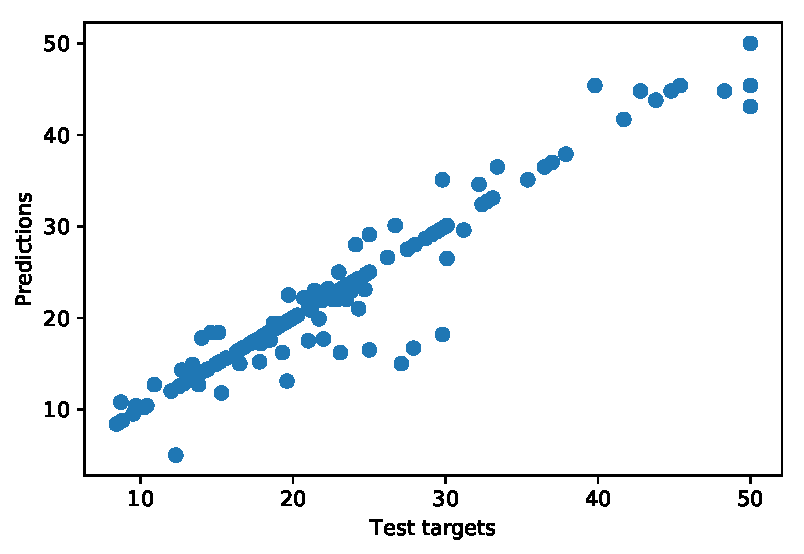
\includegraphics[width= \linewidth]{figures/RFDeconstructed_figure6_1.pdf}
\end{document}